
\chapter{Podaci i Metode} % Main chapter title

\label{Podaci i Metode} % For referencing 



\section {Podaci}

Za metode koje prezentujemo potrebne su tri vrste informacija:
\begin{enumerate}
  \item Što više različitih proteina.
  \item Pouzdana anotacija funkcija.
  \item Informacije o funkcijama, prvenstveno međurelacije.
\end{enumerate}

Međurelacije između funkcija su bitne samo ako je potrebno grupisati ih,
ili ako je potrebno mapiranje na neku drugu nomenkulaturu funkcija.

\subsection{Podaci iz originalnog rada}

U originalnom radu \parencite{Xie2007} korišćena je  baza ručno proverenih
proteinskih sekvenci \keyword{Svis-Prot} \en{Swiss-Prot}, verzija 48 iz 2005.
Verzija 48 ima 201.560 proteina od kojih 196.326 imaju dužinu preko 40
aminokiselina (što je potrebno zbog definicije ref \ref{pdis_def}). Funkcije
pridružene proteinima izražene su \keyword{kontrolisanim vokabularom}
\en{controlled vocabulary} koga čine takozvane UniProtKB \keyword{ključne reči}
\en{keywords}. U verziji 48, UniProtKB sadrži 874 ključne reči.  Zbog
statističke značajnost posmatrane su one ključne reči kojima je bilo anotirano
barem 20 proteina, tj. 710 ključnih reči.

Proteinske sekvence u Svis-Prot bazi ''nisu redundantne'' u smislu da jedan
unos u bazi predstavlja produkt jednog gena iz jedne vrstu organizma
\parencite{nonRedundant}. Zbog toga se unosi u bazu tretiraju kao proteini a ne
pojedinačne proteinske sekvence\footnote{Informacije o izomerima kao i
istorijii promena entiteta takođe se čuvaju}.  Međutim za analizu funkcija
Svis-Prot \keyword{jeste statistički redundantna} jer sadrže jako mnogo
\keyword{homologih} proteina (prvenstveno ortologa).  Originalni autori
\parencite{Xie2007} su izvršili klasterovanje Svis-Prot proteina u
\keyword{proteinske familije} dobivši 27.217 familija. Svaki protein onda ima
težinu kojom doprinosi daljoj analizi. Težina svakog proteina je inverzno
proporcionalna veličini klastera kome pripada tako da je zbir težina svih
proteina jednog klastera jednak jedan.  U našem radu nismo imali potrebe za
klasterovanjem pa nećemo dalje opisivati posledice ovog pristupa na analizu.

\textbf{komentar:} \\
Ono što autori nisu elaborirali jeste da početni uslov od minimum 20 proteina
po ključnoj reči možda nije dovoljan. Ako pretpostavimo zarad ilustracije
normalnu raspodelu veličina klastera proteina, očekivali bi da klaster najčešće
sadrži 7 proteina. Dakle iako je 50 proteina pridruženo nekoj funkciji ona
verovatno ima pridruženih svega 7 familija proteina. Kako familija sadrži
proteine pod pretpostavkom istog evolutivnog porekla njihova funkcija bi
trebalo da je slična pa se onda postavlja pitanje da li je 7 familija dovoljno
da bi se razmatrala data ključna reč. Ovo je primarno kritika za ključne reči
jer one obično predstavljaju jako opšte pojmove.

Sa druge strane za usko specijalizovane pojmove bila bi dovoljna jedna familija
proteina jer bi ona predstavljala sve razne homologe (TODO Burkhard Rost,
Termofili)

\subsection{Naši podaci}

U ovom radu korišćen je skup proteina preuzet sa \keyword{CAFA3} takmičenja.
Ovaj skup je namenjen da bude trening skup za predikciju funkcija proteina
\parencite{CAFA}.  CAFA3 trening skup je pažljivo odabran podskup Svis-Prot
proteina i smatra se da \keyword{nije statistički redundantan} \parencite{??}.
Iz tog razloga nije potrebno vršiti klasterovanje i analiza je jednostavnija te
u metodama predstavljamo samo uprošćen oblik formula.  .  Svis-Prot proteini su
kodirani jednim karakterom koristeći \keyword{IUPAC} kodove.  U podacima
postoje sekvence sa nestandardnim aminokiselinam 'U' i 'O' ili višeznačnim
oznakama 'B', 'J', 'X' i 'Z'.  Ovakve sekvence nisu podržane u našoj analizi i
za nas predstavljaju nevalidne proteinske sekvence. Pod \keyword{validnom
proteinskom sekvencom} smatraćemo sekvencu koja je validan ulaz za prediktor u
našoj analizi, tj. sačinjena je od azbuke od 20 standardnih aminokiselina i ima
najmanju dužinu 9\footnote{ Dužina 9 je minimum za VSL2b prediktor koji
koristimo}.

CAFA3 Podaci se sastoje od dve datoteke:
\begin{enumerate}
  \item \file{uniprot\_sprot\_exp.fasta}  sadrži 66.841 protein od kojih 66.599
    za našu analizu predstavljaju validnu proteinsku sekvencu . Od preostalih
    proteina njih 66.063 ima dužinu veću ili jednaku od 40 aminokiselina.
  \item \file{uniprot\_sprot\_exp.txt} pridružuje funkcije označene kao
    \keyword{GO termini} \en{Gene Ontology terms}. Postoje termini iz sve tri
    ontologije: 16.117 ćeliskih komponenti, 5.966 molekulskih funkcija i 16.117
    bioloških procesa. Jednom proteinu može biti pridruženo više GO termina i
    obrnuto.
\end{enumerate}

Naša analiza primarno je orijentisna na korišćenje GO termina za opis funkcije
i razlikuje se od originalnog pristupa.  Analiza sa GO terminima (grupisanje po
funkciji) zahteva prvenstveno poznavanje \textit{IS\_A} roditeljske veze između
termina. Takođe tokom istraživanja bile su nam potebne i ostale informacije o
terminima. Pomenute informacije dobili smo iz
\url{http://purl.obolibrary.org/obo/go.obo} dokumenta verzije 2017-12-01.

Radi poređenja dobijenih rezultata potrebno je poznavanje relacije između
ključnih reči i GO termina. Postoje dva dostupna mapiranja:
\begin{itemize}
  \item \url{www.uniprot.org/docs/keywlist.txt} verzija 20.12.2017 sadrži
    detaljan opis 1188 ključnih reči od kojih 195 pripada kategoriji
    \keyword{Molekulsih funkcija}.  Od 195 samo 145 ima mapiranje na jedan ili
    više GO termina.
  \item \url{ttp://geneontology.org/external2go/uniprotkb_kw2go} sadrži samo
    mapiranja i generiše ih \keyword{GOA projekat} \parencite{Barrell2009}.
    Ipak ova mapiranja nismo koristili jer ... \keyword{TODO}
\end{itemize}

Pošto je originalni rad \parencite{Xie2007} iz 2007. godine postoji razlike u
vokabularu ključnih reči, razlike u samim sekvencama proteina, broj proteina i
razume se anotacije ključnih reči na proteine.  Iz tog razloga bilo je potrebno
prvo ponoviti analizu sa vokabularom ključnih reči da bi se procenilo koliko
ove razlike utiču na originalne rezultate. Moramo istaći da nismo bili u
mogućnosti da proverimo ove inforamcije originalnim metodama i da priznamo da
neke razlike mogu da postoje zbog korišćenja CAFA3 statistički ne redundantnih
proteina. Međutim svako poklapanje sa originalnim rezultatima takođe potvrđuje
validnost izbora CAFA3 proteina kao dobrog statističkog uzorka.

Odlučili smo da CAFA3 podatke ne posmatramo kao crnu kutiju već da ih povežemo
sa Svis-Prot proteinima prvenstveno zbog pridruživanja ključnih reči.  kako
razlike između najnovije verzije Svis-Prot baze i CAFA3 podatak postoje bilo je
neophodno izvršiti ''korektno'' spajanje i analizu razlika. U ovom koraku
izgubili smo ?? proteina. Ovaj korak biće detaljno opisan u implementiciji.

Informacija o pridruženim ključnim rečima takođe su nam bile značajne za
proveru validnosti mapiranja na GO termine i testiranje potencijalnih drugih
metoda mapiranja. Naša je očekivanje da iste funkcije podrazumevaju
anotaciju na iste proteine.


\section {Metod}

Cilj rada je ispitivanje veze između molekulske funkcije proteina i njegove
(ne)uređenosti tj. da li molekulska funkcija zavisi više od uređenosti ili
neuređenosti.

\textbf{Idealan slučaj.} 
Pretpostavimo da za proizvoljnu molekulsku funkciju znamo sve različite
proteine koji je obavljaju.  Da bi dali korektan odgovor  moramo da znamo kako
neuređenost pojedinačnog proteina utiče na ponašanje protein.  Zatim moramo da
znamo da li i kako to ponašanje (tip neurđenosti) utiče na datu funkciju.
Nažalost kao i 2006. ni danas ovakve informacije nisu dostupne.

\textbf{Realnost.} 
\begin{itemize}
  \item Broj eksperimentalno određenih neuređenih regiona je jako mali.
    \keyword{Disprot baza} eksperimentalno utvrđenih neuređenih regiona ima
    svega 803 proteina sa opisanih 2167 neuređenih regiona. Još gore pouzdanost
    ovih regiona je diskutabilna jer različite eksperimentalne tehnike koje su
    korišćene imaju različitu pouzdanost. Najveću pouzdanost nose regioni koji
    su eksperimentlano utvrđeni sa što većim brojem pouzdanih eksperimentalnih
    tehnika \parencite{disprot}. 
  \item Prediktori su trenirani na malom podskupu proteina (Disprot, PDB, ...).
    Čak i konsenzus nekoliko različitih prediktora ne daje dovoljno pouzdane
    rezultate o lokciji neuređenog regiona\parencite{Mitic}.
  \item Koliko nam je poznato trenutno nema prediktora koji predviđaju tip
    neuređenosti. Takođe Opisivanje tipa neuređenosti predstavlja poduhvat.
    \begin{itemize}
      \item Prof. Vladimir Uverski predlaže nekoliko imena za opis različitih
        ponašanja neuređenih proteina \en{Folldon, Unfolldon, ...}
        \parencite{Uversky2017}.
      \item Prof. Peter Tompa je zaslužan za kreiranje 3 ontologije neuređenih
        regiona za bazu Disprot koji precizno modeluje tipove
        neuređenosti\parencite{disprot}.  .  Međutim koliko nam je poznato
        prediktori koji predviđaju termine ove ontologije još nisu napravljeni
    \end{itemize}

\end{itemize}

Jedina alternativa jeste da se predpostavi da veći udeo neuređenih u odnosu na
uređene proteine podrazumeva da funkcija zavisi više od neuređenosti.  Dakle
izjednačićemo uzročnost \en{causation} i \keyword{korelaciju}. Ali prvo
potrebno je definisati kada protein smatramo neuređenim.  Definicija mora da
ima biološkog smisla, da bude prilagođena analizi ali pored toga ograničena je
sposobnostima i preciznošću prediktora koji se korist.  Više o tome u nastavku.


\subsection{Predikcija neuređenosti proteina}

Autori \parencite{Xie2007} koristili su \keyword{PONDR VL3E} prediktor koji
postiže tačnost od $~87\%$ pri unakrsnoj validaciji nad uravnoteženim test
skupom.  Zbog ekonomičnosti i dostupnosti mi smo koristili noviji prediktor
\keyword{PONDR VSL2b}.

Oba prediktora pripadaju \keyword{PONDR} \en{(Predictor Of Naturally Disordered
Regions)} familiji prediktora. Ovi prediktori zasnivaju se na eksperimentalno
pokazanim karakteristikama neurđenih regiona. Preciznije određene aminokiseline
verovatnije su da se jave u neuređenom regionu. Neuređeni regioni imaju manje
aromatičnih i hidrofobnih AK, veći ukupni naboj, veći indeks fleksibilnosti i
manju kompleksnost sekvence. Ove osobine izražene kao atributi koriste se za
treniranje neuronske mreže sa propagacijom unapred \en{ feed forward neural
networks } koja koristi prozor veličine između 9 i 21 aminokiseline.
Finalni prediktor predstavlja kombinaciju nekoliko neuronskih mreža gde je
svaka od njih trenirana nad različitim podacima specijalizujući se da predviđa
samo regione određene veličine ili položaja. PONDR familija ima nekoliko
prediktora koji  se razlikuju u načinu treniranja što se postiže kombinacijom
različitih trening skupova.  Oznaka ''VSL2b'' kodira tipove proteinskih trening
skupova.
\begin{itemize}
  \item V - Opisuje eksperimentalnu tehniku kojom je neurđenost utvrđena na
    trening skupu \en{X-ray, NMR, circular dichroism}
  \item S - Prediktor je treniran na skupu proteina sa \keyword{kratkim}
      neruređenim
    regionim ($<30$ AK)
  \item L - Prediktor je treniran na skupu proteina sa \keyword{dugim}
    neuređenim regionima ($>30$ AK)
\end{itemize}

VSL2b kao ulaz prima proteinsku sekvencu minimalne dužine 9 AK kodiranih jednim
karakterom. Podržava azbuku od samo 20 standardnih AK.  Izlaz je niz
ocena(verovatnoća) za svaku aminokiselinu da li pripada neuređenom regionu to
jest da je taj rezidual
\footnote{ Rezidual je čest naziv koji se koristi za aminokiseline i nukleinske
  kiseline na nekoj poziciji sekvence.  Naziv potiče od hemiskih tehnika
  prečišćavanja čiji su rezultati reziduali (ostaci).
} neuređen. Reziduale sa vrednošću iznad 0.5 smatramo neuređenim a suprotno
uređenim. Za potrebe analize autori \parencite{Xie2007} uvode sledeću definiciju.

\newtheorem{mydef}{Definicija}
\begin{mydef}
\label{pdis_def}
Protein je \keyword{verovatno/putativno neuređen} \en {putatively disordered}
ako sadrži bar jedan region veći ili jednak od 40 uzastopnih aminokiselina
takvih da imaju \textit{predviđenu neuređenost} iznad 0.5. 
\end{mydef}

Onda definišemo operator $d$ takav da za svaku proteinsku sekvencu $s_i$ važi:


\[   
  d(s_i) = 
    \begin{cases}
      1 & \text{ako je} \quad s_i \quad \keyword{verovatno neuređena}\\
      0 & \text{suprotno}
    \end{cases}
\]

Uslov ''$\ge40$'' u originalnom radu delom je posledica ograničenja VL3
prediktora koji je treniran na \keyword{dugim} sekvencama. Mi nismo u obavezi
da sledimo ovo pravilo ali to radimo radimo radi upoređivanja rezultata.


\subsection{Zavisnost dužine proteina i predikcije dugačkog neuređenog regiona}

Verovatnoća da po gornjoj definiciji protein bude klasifikovan kao verovatno
neuređen raste sa porastom njegove dužine. Ovo je ozbiljan problem koji utiče
na statističku značajnost rezultata. Autori \parencite{Xie2007} 
predlažu narednu formulu da se ta verovatnoća proceni:

Neka $S_L$ skup proteina sa dužinama između $[L-l, L+l]$ gde je $l
= 0.1*L$. Dobijamo sledeće formule:

$$ S_L = \{s_i \mid \quad | L -  \Vert s_i \Vert | <= l \quad   \}$$
$$ P_L = \dfrac{ \sum_{s_i \in S_L} d(s_i)} {\Vert S_L \Vert}$$

Ponašanje $P_L$ predstavljeno je na grafiku \ref{fig:PL1}. Glatkoća rezulatata
kontroliše se veličinom $l$ koja predstavlja prozor uprosečavanja. Kako prozor
uglačavanja raste sa porastom dužine proteina $(l = 0.1*L)$
tako da prozor uprosečavanja raste sa porastom dužine proteina te $P_L$
postaje glađe sa veličinom proteina. Za konstantni prozor uprosečavanja ova
tehnika je još poznata kao \en{rolling average} ili \en{boxcar filter} i
pripada specijalnoj vrsti konvolucije. \keyword{Trenutno ne znamo zašto se
autor odlučio da veličina prozora raste sa dužinom proteina???}.


\begin{figure}[th]
\centering
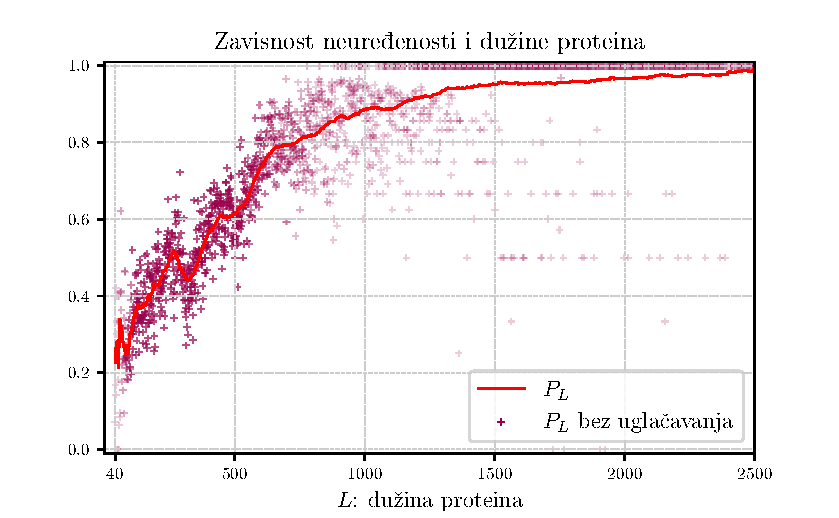
\includegraphics[]{plots/PL_F}
\decoRule
\caption {
 Punom linijom predstavljena je $P_L$ sa prozorom uprosečavanja $l = 0.1L$,
 a krstići predstavljaju sirove vrednosti $l = 0$ 
}
\label{fig:PL1}
\end{figure}


Pored gore prikazanog 'originalnog' metoda predstavljamo još jedan pristup.
\keyword{Slučajno generisani} \en{random generated} proteini za procenu $P_L$.
Razmotrićemo dva modela. Prvi je naivan model \keyword{uniformne verovatnoće}
koji podrazumeva da se svaka aminokiselina javlja sa istom verovatnoćom odnosno
$1/20$. U statistici ovo je još poznato kao \en{equiprobable model}.  Drugi
model koji ćemo zvati 'slučajni' ili 'random' model predstavlja slučajnu
promenljivu čija verovatnoća zavisi od učestalosti aminokiselina iz CAFA3 skupa
i prikazana je na grafiku \ref{fig:AK_ucestalost}.  Koristeći ova dva modela za
svaki protein generisan je slučajan protein iste dužine koji se koristi za
procenu $P_L$.


\begin{figure}[th]
\centering
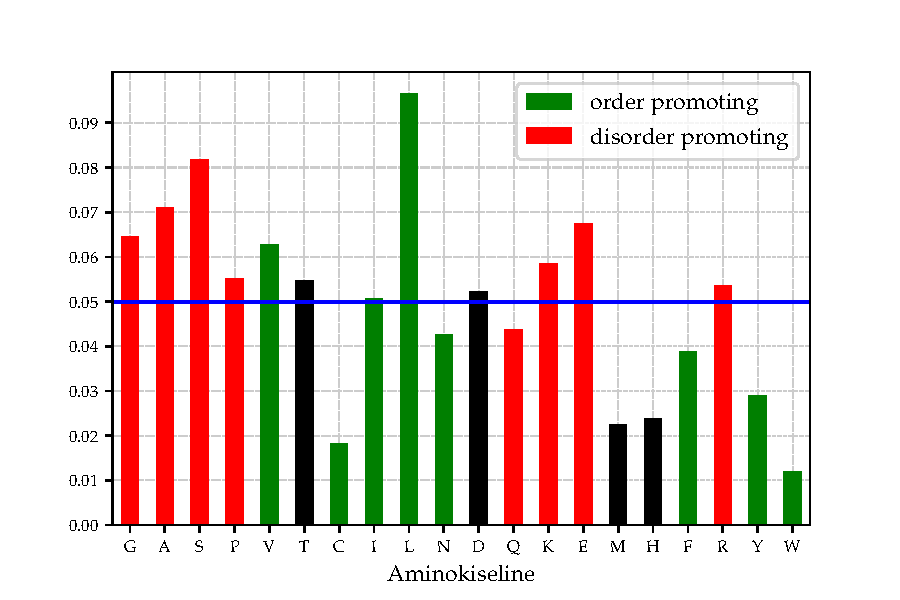
\includegraphics[]{plots/AK_ucestalost}
\decoRule
\caption{Slučajni i uniformni modeli za procenu $PL$}
\label{fig:AK_ucestalost}
\end{figure}



Poređenje ova dva pristupa sa originalnim $P_L$ prikazano je na slici
\ref{fig:PL2}.  Originalni $P_L$ ostaje prikazan kao puna linija. Jasno se vidi
da slučajni model prikazan isprekidanom linijom predstavlja vizuelno dobru
aproksimaciju dok uniformni model verovatnoća prikazan tačkicama znatno odstupa
i dosta sporije raste (reklo bi se skoro linearno). Kako VSL2b predkitor
prepoznaje neuređene regione na osnovu učestalosti aminokiselina ovo ponašanje
nije čudno jer je manja verovatnoća pojave aminokiselina koje promovišu
neuređenost. Zbog suviše velikog odstupanja uniformni model nije korišćen u
daljoj analizi.


\begin{figure}[th]
\centering
% 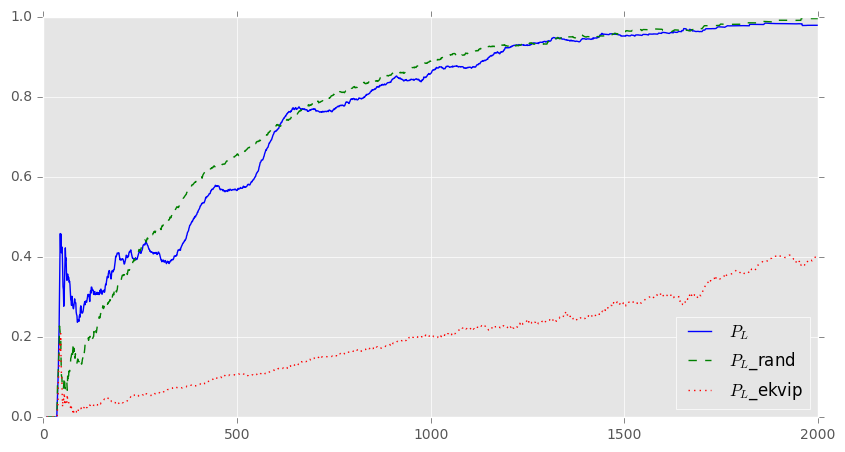
\includegraphics[scale=0.65]{Figures/PL2}
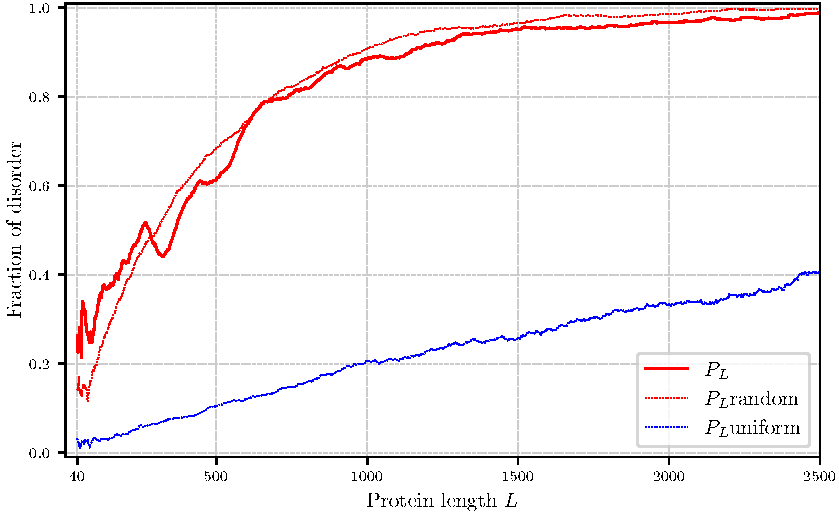
\includegraphics[]{plots/PL_F_cmp}
\decoRule
\caption{Različiti pristupi za procenu $P_L$}
\label{fig:PL2}
\end{figure}


Jedno objašnjenje zašto je uniformni model naivan i toliko odstupa od
prvobitnog metoda proizilazi iz činjenice da aminokiseline imaju inherentno
različite verovatnoće. Naime  aminokiseline ne mogu  imati istu
verovatnoću jer se  broj njihovih kodona razlikuje. Neke aminokiseline
su kodirane sa samo jednim a druge i sa 6 kodona. Očekivali bi da broj kodona
povećava učestalost aminokiseline i ta korelacija uz izuzetke arginina se vidi
na slici
\ref{fig:aminoacid} \parencite{AKfrekvencija}.

\begin{figure}[th]
\centering
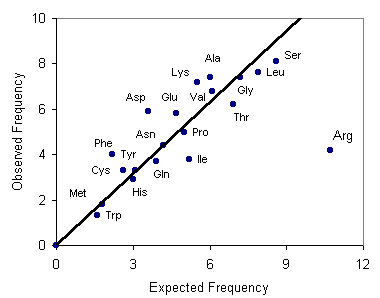
\includegraphics[scale=0.7]{aminoacid}
\decoRule
\caption{očekivana i realna učestalost  aminokiselina kod sisara}
\label{fig:aminoacid}
\end{figure}



\subsection{Ocenjivanje zavisnosti funkcije od neuređenosti}

Neka je $S_j$ skup proteina koji imaj pridruženu funkciju $j$. Tada se procenat
verovatno neuređenih proteina u oznaci $F_j$ može izračunati kao: $$F_j =
\dfrac{\sum_{s_i \in S_j} d(s_i)} {\Vert S_j \Vert} $$

Nultu hiptezu koja predviđa da je rezultat $F_j$ posledica samo slučajnosti, to
jest zavisi samo od $P_L$ opisana je preko slučajne veličinu $Y_j$
gde je $X_L$ Bernulijeva slučajna veličina sa verovatnoćom $P(X_L = 0) = P_L$
odnosno $P(X_L = 1) = 1-P_L$

$$ Y_j = \dfrac {\sum_{s_i \in S_j} {X_{|s_j|}}}{\Vert S_j \Vert}$$

Ako $F_j$ izlazi iz intervala poverenja raspodele $Y_j$ onda funkcija $j$
sadrži značajno mnogo predviđenih neuređenih ili uređenih proteina. Preciznije
ako je \textit{p-value} $<0.05$ funkcija $j$ je povezana sa neuređenim
proteinima a ako je \textit{p-value} $>0.95$ funkcija $j$ je povezana sa
uređenim proteinima. Suprotno ne može ništa da se tvrdi za funkciju $j$.

$Y_j$ je teško izračunati analitički te mora da se pribegne empiriskom
računanju p-vrednosti. Empiriska p-vrednost određena je tako što je za 1000
realizacija $Y_j$ izračunato očekivanje da je realizacija $Y_j$ veća od $F_j$.
\begin{verbatim}
    p = np.array( [yj>Fj for yj in Yj_1000] ).mean()
\end{verbatim}
U radu \parencite{Xie2007} autori tvrde se da za veće skupove $S_j$ raspodela
$Y_j$ ponaša kao normalna pa se ocena Z-skor može dobiti kao
$Z_j=(F_j-\mu_j)/\delta_j$ gde je $\mu_j$ očekivanje a $\delta_j$ standardna
devijacija.  Dodatno p-vrednost može da se aproksimira kao $1/2(1-erf(Z_j/2))$
\footnote{$erf()$ je gausova funkcija greške,
$erf(x)=\dfrac{2}{\sqrt{\pi}} \int_{0}^{x}  e^{-t^2} dt$ }
ako raspodela liči na normalnu. Ovo je nekad korisno jer sa 1000 realizacija
$Y_j$ nema dovoljnu preciznost za p vrednost manju od $1/1000=0.001$. Međutim u
ovom radu to nije korišćeno jer su sva sortiranja(kao i u originalnom radu)
izvršena po Z-skor oceni.


